\chapter{量子算法 (Quantum algorithms)}

在全书的开篇第 1 章中，我们曾见证了一个深刻的对比：素性测试可以在多项式时间内高效解决，而质因数分解却极其困难——在传统经典计算机上已知最快的方法都需要耗费输入规模指数级的时间。正是因数分解的这种计算难解性，构成了现代互联网公钥密码学（如 RSA）的坚固基石。

在本章中，我们将迎来全书的最高潮：\textbf{质因数分解在量子计算机上可以在多项式时间内被彻底破解}！这就是彼得·秀尔（Peter Shor）在 1994 年提出的著名的 Shor 量子分解算法。

\section{量子比特、叠加态与测量 (Qubits, superposition, and measurement)}

经典计算机的基本信息单元是比特（Bit），其状态非 0 即 1。而量子计算的基本单元是\textbf{量子比特 (Qubit)}。

\subsection*{量子叠加态 (Superposition)}
一个量子比特的状态可以处于 $|0\rangle$ 和 $|1\rangle$ 的线性叠加之中：
\[
|\psi\rangle = \alpha |0\rangle + \beta |1\rangle,
\]
其中 $\alpha, \beta \in \mathbb{C}$ 为复数概率幅（Amplitudes），满足归一化条件：
\[
|\alpha|^2 + |\beta|^2 = 1.
\]

对于一个包含 $n$ 个量子比特的系统，其量子态是 $2^n$ 个基态的叠加：
\[
|\psi\rangle = \sum_{x \in \{0, 1\}^n} \alpha_x |x\rangle, \quad \text{满足} \quad \sum_{x \in \{0, 1\}^n} |\alpha_x|^2 = 1.
\]
仅需 500 个量子比特，其叠加态向量的维度就超过了已知宇宙中所有基本粒子的总数！

\subsection*{量子测量 (Measurement)}
当对量子态 $|\psi\rangle$ 进行物理测量时，叠加态将瞬间发生\textbf{波函数坍缩}：系统以概率 $|\alpha_x|^2$ 坍缩为具体的某个经典基态 $|x\rangle$。

\begin{sidebarbox}{量子纠缠 (Entanglement)}
若两个或多个量子比特构成的复合系统状态无法分解为各自独立量子比特状态的张量积（例如著名的 EPR 贝尔态 $|\Phi^+\rangle = \frac{1}{\sqrt{2}}|00\rangle + \frac{1}{\sqrt{2}}|11\rangle$），则称这些量子比特之间存在\textbf{量子纠缠}。对其中一个粒子的测量将瞬间决定远在光年之外的纠缠伴侣的状态。
\end{sidebarbox}

\section{量子傅里叶变换 (The quantum Fourier transform, QFT)}

在第 2 章中，我们见识了经典快速傅里叶变换（FFT）如何在 $O(n \log n)$ 时间内完成离散傅里叶变换。而在量子计算中，\textbf{量子傅里叶变换 (QFT)} 能够在一组大小为 $M = 2^m$ 的量子叠加态基底上，在仅仅 $O(m^2) = O(\log^2 M)$ 步量子逻辑门操作内完成傅里叶变换！

QFT 将基态 $|x\rangle$ 变换为：
\[
\text{QFT} |x\rangle = \frac{1}{\sqrt{M}} \sum_{y=0}^{M-1} \omega^{xy} |y\rangle, \quad \text{其中 } \omega = e^{2\pi i / M}.
\]
QFT 是一个酉矩阵变换（Unitary transformation），它能够使不同计算路径上的概率幅发生\textbf{相长干涉 (constructive interference)} 或\textbf{相消干涉 (destructive interference)}。

\begin{figure}[htbp]
\centering
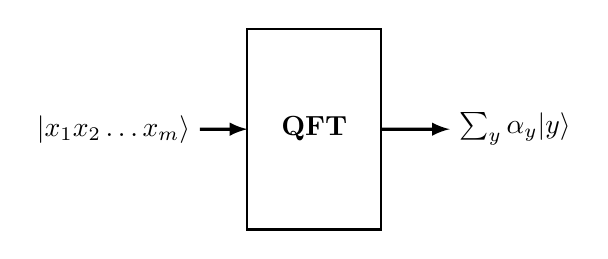
\begin{tikzpicture}[scale=0.85, >=latex]
    \node (in) at (0,1.5) {$|x_1 x_2 \dots x_m\rangle$};
    \draw[thick] (2,0) rectangle (4,3);
    \node at (3,1.5) {\textbf{QFT}};
    \node (out) at (6,1.5) {$\sum_y \alpha_y |y\rangle$};
    
    \draw[->,very thick] (in) -- (2,1.5);
    \draw[->,very thick] (4,1.5) -- (out);
\end{tikzpicture}
\caption{量子傅里叶变换电路的宏观抽象}
\label{fig:qft_block}
\end{figure}

\section{周期性寻找 (Periodicity)}

假设我们有一个周期函数 $f(x)$，其周期为 $r$（即 $f(x + r) = f(x)$）。在经典计算中寻找黑盒函数的周期需要指数次函数查询。

但在量子计算机上，寻找周期的步骤如下：
\begin{enumerate}
    \item 准备两组量子寄存器，初始化为均匀叠加态：
    \[
    \frac{1}{\sqrt{M}} \sum_{x=0}^{M-1} |x\rangle |0\rangle;
    \]
    \item 评估量子黑盒函数 $U_f$，将状态演化为：
    \[
    \frac{1}{\sqrt{M}} \sum_{x=0}^{M-1} |x\rangle |f(x)\rangle;
    \]
    \item 测量第二个寄存器，得到某个值 $f(x_0)$。此时第一个寄存器瞬间坍缩为所有满足 $f(x) = f(x_0)$ 的等间距周期基态的叠加：
    \[
    \sum_{k} |x_0 + k r\rangle;
    \]
    \item 对第一个寄存器执行\textbf{量子傅里叶变换 (QFT)}：由于傅里叶变换将周期为 $r$ 的脉冲梳转换为频域中间隔为 $M/r$ 的干涉尖峰，所有概率幅高度集中在 $M/r$ 的整数倍上；
    \item 测量第一个寄存器并利用连分数展开，即可高概率直接提取出周期 $r$！
\end{enumerate}

\section{因数分解归结为求周期 (Factoring as periodicity)}

如何利用量子周期寻找算法来分解大整数 $N$？数论为我们提供了架向目标的桥梁：
\begin{enumerate}
    \item 随机选取一个与 $N$ 互质的整数 $x < N$；
    \item 考虑模幂函数 $f(a) = x^a \bmod N$。由欧拉定理可知，该函数是一个周期函数，其周期 $r$ 满足 $x^r \equiv 1 \pmod N$（即 $x$ 模 $N$ 的阶）；
    \item 使用量子算法在多项式时间内求出周期 $r$；
    \item 若 $r$ 为偶数，则：
    \[
    x^r - 1 = (x^{r/2} - 1)(x^{r/2} + 1) \equiv 0 \pmod N.
    \]
    这意味着 $(x^{r/2} - 1)(x^{r/2} + 1)$ 是 $N$ 的倍数。
    \item 计算 $\gcd(x^{r/2} - 1, N)$ 以及 $\gcd(x^{r/2} + 1, N)$，有极高概率直接获得 $N$ 的非平凡质因子！
\end{enumerate}

\begin{theorem}[\textbf{Shor 质因数分解定理}]
利用量子傅里叶变换与周期寻找，可以在 $O(n^3)$ 的多项式量子门操作时间内分解一个 $n$ 位的正整数 $N$。
\end{theorem}

\begin{sidebarbox}{对计算机科学与物理学的深远影响}
Shor 算法在学术界引发了地震：它首次无可辩驳地证明了量子力学规律所支持的计算模型（BQP）严格超越了基于图灵机的传统经典计算模型（BPP）。人类对“何为有效可计算”的认知边界被永远地改写了。
\end{sidebarbox}

\newpage
\section*{习题 (Exercises)}
\addcontentsline{toc}{section}{习题}

\begin{exercise}{10.1}
计算 Hadamard 门 $H = \frac{1}{\sqrt{2}}\begin{pmatrix} 1 & 1 \\ 1 & -1 \end{pmatrix}$ 作用在基态 $|0\rangle$ 和 $|1\rangle$ 上的输出状态。
\end{exercise}

\begin{exercise}{10.2}
受控非门（CNOT 门）的真值表与其在生成纠缠贝尔态中的作用。
\end{exercise}

\begin{exercise}{10.3}
证明量子不可克隆定理（No-Cloning Theorem）：不存在能够复制任意未知量子态的酉变换操作。
\end{exercise}

\begin{exercise}{10.4}
Deutsch-Jozsa 算法：用单次量子黑盒查询判断布尔函数是常数函数还是平衡函数。
\end{exercise}

\begin{exercise}{10.5}
推导 4 个基态上的量子傅里叶变换矩阵 $M_4(\omega)$ 与经典 4 点 FFT 矩阵的对应关系。
\end{exercise}

\begin{exercise}{10.6}
Simon 周期寻找问题：在量子多项式时间内求解 XOR 异或周期隐藏子群问题。
\end{exercise}

\begin{exercise}{10.7}
使用连分数展开（Continued Fractions）从测量的频域峰值精确重构周期 $r$。
\end{exercise}

\begin{exercise}{10.8}
Grover 量子无序数据库搜索算法：在 $O(\sqrt{N})$ 时间内完成非结构化数据库搜索。
\end{exercise}
